% !TEX encoding = UTF-8 Unicode
\documentclass[a4paper,10pt]{article}
\usepackage[utf8]{inputenc}
\usepackage{listings}
\usepackage[francais]{babel}
\usepackage[T1]{fontenc}
\usepackage{graphicx}
\usepackage{caption}

\author{Présent: Tous}
\title{PV réunion 1}
\date{5 décembre 2013}

\begin{document}
\maketitle
\part*{Définition des acteurs}
\begin{enumerate}
\item[•] Joueur : Personnage fictif appartenant à une équipe. A un inventaire (liste(?)) avec au moins un balais.
\item[•] Client : Processus s'exécutant sur la machine d'un utilisateur.
\item[•] Serveur : Processus s'exécutant sur un serveur
\item[•] Jeu
\item[•] Equipe : Possède 7 joueurs
\item[•] Manager (Utilisateur/User)
\item[•] Installation : Element améliorable du club
\item[•] Club
\item[•] Match
\item[•] Terrain
\item[•] ScoreBoard
\end{enumerate}
\part*{Notes sur le srd}
\begin{description}
\item[Historique du document : ]Définir avec Github et pv, /!\textbackslash{} Fournir le nom de(s) autheur(s) pour chaque version
\item[Besoin système - Exigences fonctionnelles : ]Multithreéding -> 1 thread par user et par match
\item[Design et fonctionnement du système : ]Mettre les diagrammes
\end{description}
\part*{Schémas}
\begin{description}
\item[\LARGE Use Case (Client)] :\\
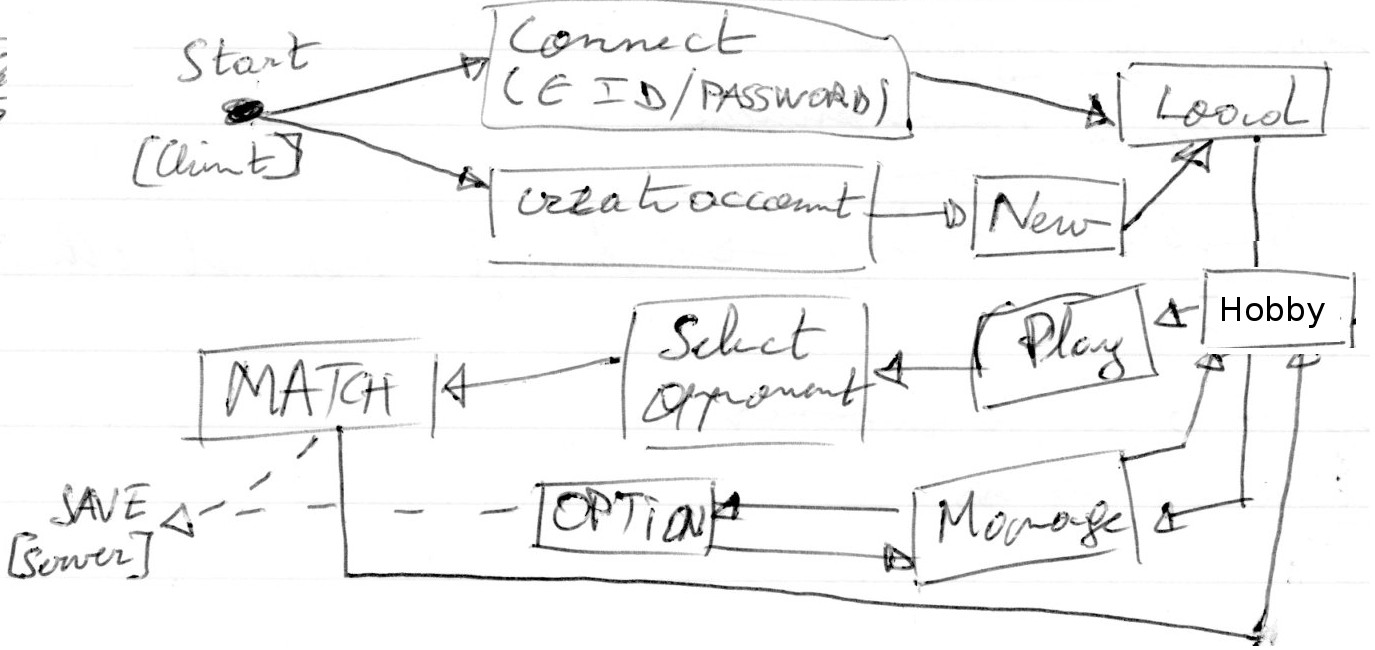
\includegraphics[scale=1]{schema1_pv1.jpg}
\item[\LARGE Class Diagram (Club)] :\\
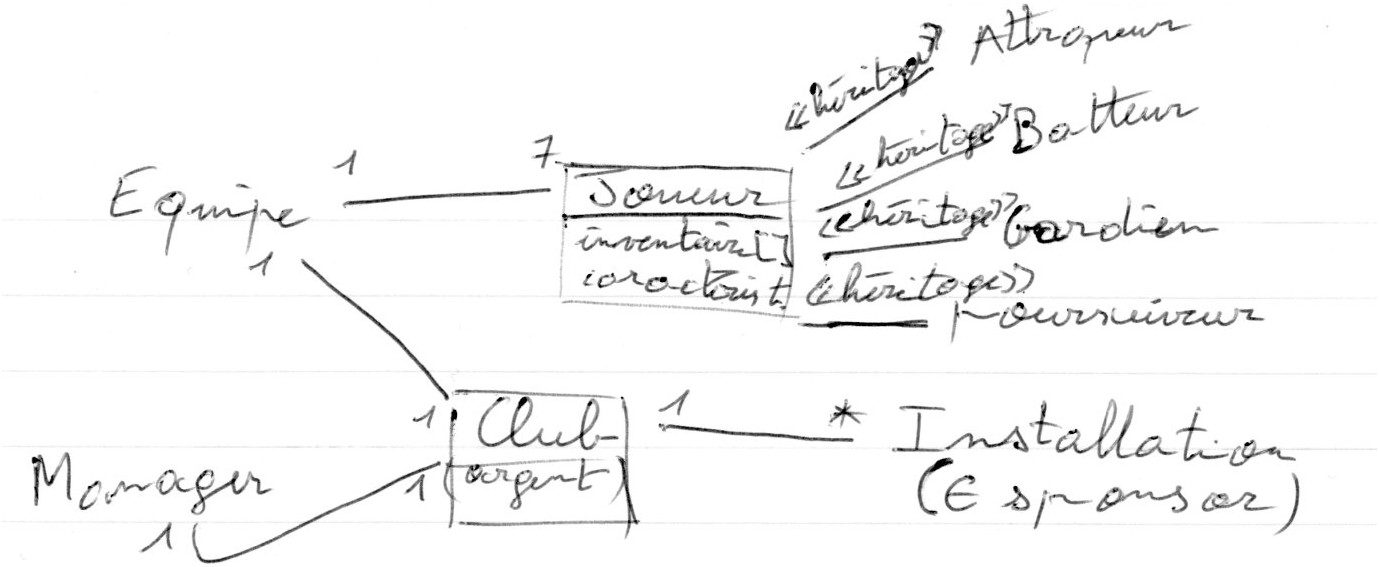
\includegraphics[scale=1]{schema2_pv1.jpg}
\newpage
\item[\LARGE Class Diagram (Match)] :\\
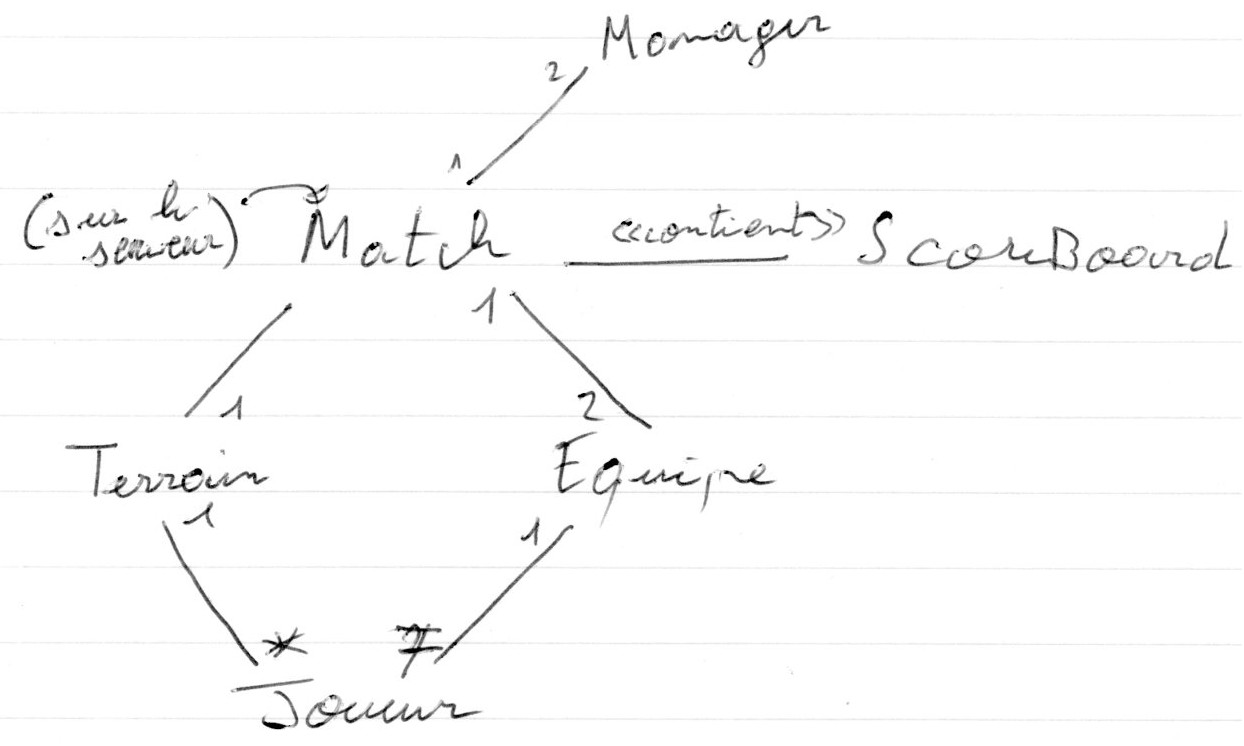
\includegraphics[scale=1]{schema3_pv1.jpg}
\end{description}
\part*{Idée pour le terrain}
\begin{figure}[!h]
\centering
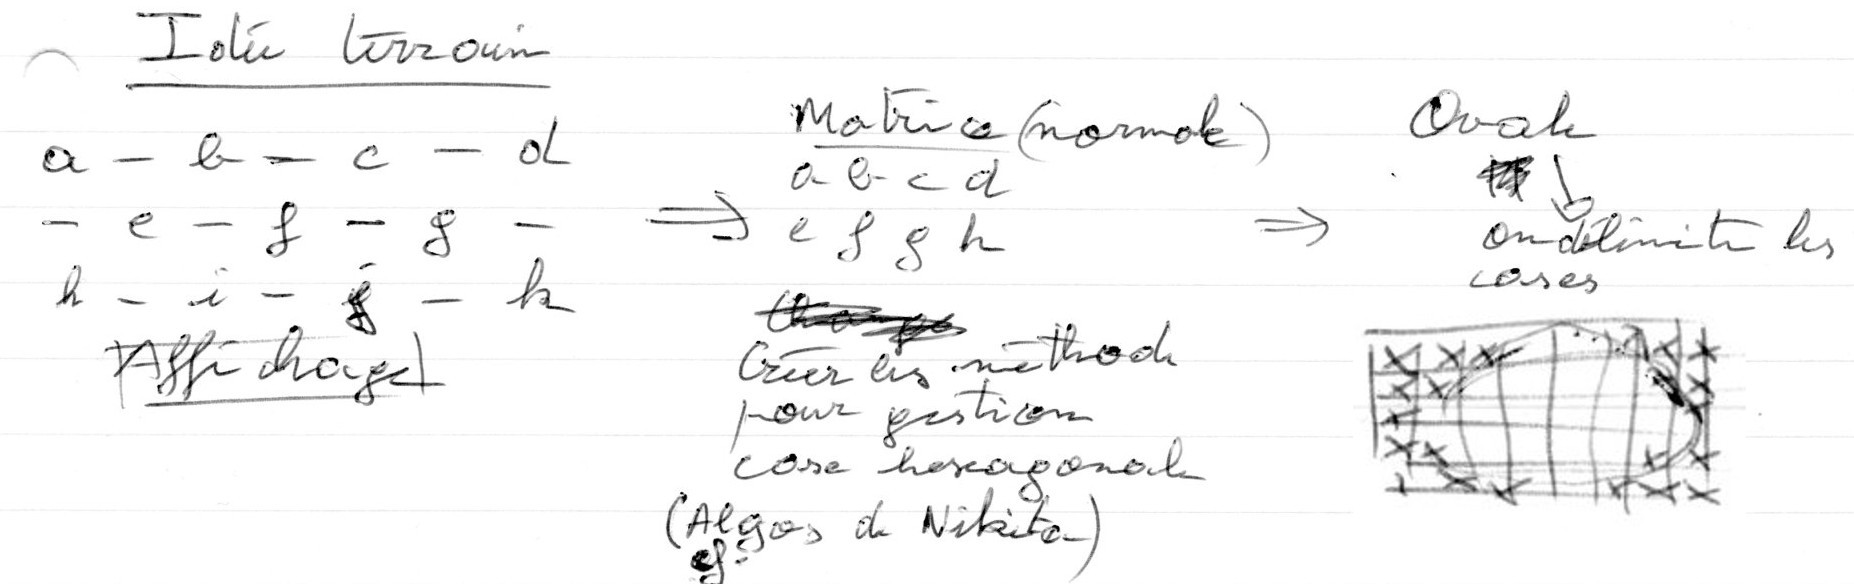
\includegraphics[scale=0.8]{schema4_pv1.jpg}
\caption{Affichage et représentation du terrain}
\end{figure}
Idée : Gestion auto-save en match via JSON (objet se comportant comme des dictionnaires (?) avec du texte) -> débug + facile \\
On redessine tout à chaque changement, chez le client\\
/!\textbackslash{} Le joueur ne peut être bougé que si le serveur l'authorise (le client demande -> le serveur vérife -> si OK, on bouge le joueur et on affiche le changement chez le client, sinon on renvoie un message)
\part*{Organisation}
\begin{description}
\item Langage à utiliser : c/c++
\item Communication par Skype
\item Code par Github
\item LaTeX pour le rapport/srd
\item ArgoUML pour les diagrammes
\item N.B.: Nikita se propose pour les tests
\item 
\item 
\item \LARGE Prochaine réunion :\\ le 6 décembre à 11h devant la cafétaria
\end{description}
\end{document}